\documentclass{article}

\usepackage{physics} % Handy shortcuts like \pdv, \dd and much more
\usepackage{geometry} % smaller margins, can be adjusted if given arguments
\usepackage{siunitx} % the \si environment for units
\usepackage{mathtools} % The dcases environment, prettier than just cases
\usepackage{tikz} % For drawing pictures
\usepackage{wrapfig} % Wrapping text around figures
\usepackage{enumitem} % Getting alphabetical enumerate
\usepackage{bbold}



\title{Exercise 8 solutions - TFY4345 Classical Mechanics}
\date{2020}

\begin{document}
    \maketitle
    \section{Principal moments of inertia of a triangular slab}
        (a) Since the mas has uniform density, we can write the mass area density as $M =   1/2 ab\rho$. Let $x_{CM}$ denote the $x$-component of the center of mass. Using the definition of $CM$, we find
        \begin{equation*}
            x_{CM} = \frac{1}{M} \int_0^a \dd x \int_0^{b(1 - x / a)} \dd y \rho x = \frac{\rho b}{M} \int_0^a \dd x \left( 1 - \frac{x}{a}\right) = \frac{a^2 b \rho}{M} \int_0^1 \dd u (1 - u)u = \frac{\rho a^2 b}{6M} = \frac{a}{3}. 
        \end{equation*}
        We used the substitution $u = 1 - x/a$ which implies a $ \dd x = - a \dd u $. Because of the symmetry in the problem (the slab is a triangle), the calculation of $y_{CM}$ is the same, only exchanging $ a \leftrightarrow b $, so the result is $y_{CM}$ = b/3. 
        \\ \\
        (b) The slab is two dimensional, and laying in the $xy$-plane. If we look at the definition of the off-diagonal entries in moment of inertia tensor,
        \begin{equation*}
            I_{ij} = - \int_V \dd V x_ix_j,
        \end{equation*} $I_{zx} = I_{xz} = I_{zy} = I_{yz} = 0$, as  z = 0. This also implies that $I_{xx} + I_{yy} = I_{zz}$, so all we need to calculate is $I_{xx}, I_{yy}$ and $I_{xy}$.
        \begin{align*}
            I_{xy} =& -\rho \int_0^a \dd x \int_0^{v(1 - x/a)} \dd y yx = - \frac{\rho b^2}{2}\int_0^a \dd x x \left( 1 - \frac{x}{a} \right)^2 = - \frac{\rho b^2}{2} \int_0^a \dd x \left( x - \frac{2}{a}x^2 + \frac{1}{a^2} x^3\right) \\
            &= -\frac{\rho b^2 a^2}{2}\left( \frac{1}{2} - \frac{2}{3} + \frac{1}{4} \right) = \frac{M a b}{12} \\
            I_{xy} = & -\rho \int_0^a \dd x \int_0^{v(1 - x/a)} \dd y y^2 = \frac{\rho b^3}{3}
            \left(1 - \frac{x}{a}\right)^3 = \frac{\rho a b^3}{3} \int_0^1 \dd u u^3 = \frac{M b^2}{6}.
        \end{align*} 
        Lastly, $I_{yy}$ can a gain be found just by the exchange $a \leftrightarrow b$. In matrix form,
        \begin{equation*}
            I = \frac{M}{6}
            \begin{pmatrix*}
                b^2 & -\frac{1}{2} ab & 0 \\
                -\frac{1}{2} ab & a^2 & 0 \\
                0 & 0 & a^2 + b^2 \\
            \end{pmatrix*}
        \end{equation*}
        \\ \\
        \begin{wrapfigure}{2}{0.4\textwidth}
            \includegraphics[width=0.4\textwidth]{figures/exercise_1_triangle2.pdf}
        \end{wrapfigure}
        (c) We can remove the common factor $M/6$, so insert our values into the new variables, we get
        \begin{equation*}
            A = \frac{1}{2}(a^2 + b^2), \quad B = \frac{1}{2}\sqrt{(b^2 - a^2) +a^2b^2}, \quad \vartheta = \tan^{-1}\left( \frac{ab}{b^2 - a^2} \right).
        \end{equation*} 
        \newpage
        The last equation describes a triangle with side lengths $b^2 - a^2, \, ab$ and $\sqrt{(b^2 - a^2) +a^2b^2} = 2B$, and an angle $\vartheta$ opposite the side of length $ab$. This gives us the relations $ab=2 B \sin(\vartheta)$ and $b^2 - a^2 = 2B \cos(\vartheta)$. It follows that
        \begin{align*}
            a^2 &= \frac{1}{2}(b^2 + a^2)  - \frac{1}{2}(b^2 - a^2) = A - B \cos(\vartheta) \\
        b^2 &= \frac{1}{2}(b^2 + a^2)  + \frac{1}{2}(b^2 - a^2) = A + B \cos(\vartheta)
        \end{align*}
        Putting all this together, we get 
        \begin{equation*}
            I = \frac{M}{18}
            \begin{pmatrix*}
                A + B\cos(\vartheta) & B \sin(\vartheta) & 0 \\
                B \sin(\vartheta) & A - B\cos(\vartheta) & 0 \\
                0 & 0 & 2A
            \end{pmatrix*}
        \end{equation*}

        To find the principal moments of inertia, we must find solve the characteristic equation for the principal moments of inertia $\omega$
        \begin{align*}
             \det(I - \omega) = 0& \implies
            \begin{vmatrix*}
                A + B\cos(\vartheta) - \omega & B \sin(\vartheta) & 0 \\
                B \sin(\vartheta) & A - B\cos(\vartheta) - \omega & 0 \\
                0 & 0 & 2A - \omega
            \end{vmatrix*} \\
            &= (2A - \omega) \big[(A + B\cos(\vartheta) - \omega) (A - B\cos(\vartheta) - \omega)  - B \sin(\vartheta) \big]  \\
            &= (2A - \omega)[A^2 - B^2 + \omega^2 - 2\omega A] \\
            &= (2A - \omega)[(A - \omega)^2 - B^2] = 0,
        \end{align*}
        which has the solutions $\omega_1 = 2A, \, \omega_2 = A+B$ and $\omega_3 = A-B$. By inspection, the first eigenvector is $\mathbf{v} = (0, 0, 1)$. We can then only look at the relevant part of the matrix to find the others. Inserting $\omega = A + B $,
        \begin{align*}
            0 = & (I - \omega \mathbb{1}) \mathbf{v} = B
            \begin{pmatrix*}
                \cos(\vartheta) - 1 & \sin(\vartheta)  \\
                \sin(\vartheta) & -\cos(\vartheta)-1  \\
            \end{pmatrix*} 
            \begin{pmatrix*}
                v_1 \\
                v_2 
            \end{pmatrix*}
        \end{align*}
        Setting $v_2 = 1$, we get $v_1 = \sin(\vartheta) / (1 - \cos(\vartheta))$. The normalized eigenvector then becomes
        \begin{align*}
            \mathbf{v} &= \frac{1}{\sqrt{1 + \frac{\sin^2(\vartheta)}{(1 - \cos(\vartheta))^2}}} \left( \frac{\sin(\vartheta)}{1 - \cos(\vartheta)}, 1, 0 \right)
            = \frac{1 - \cos(\vartheta)}{\sqrt{1 - 2 \cos(\theta) + \cos^2(\vartheta)  + \sin^2(\vartheta)}}\left( \frac{\sin(\vartheta)}{1 - \cos(\vartheta)}, 1, 0 \right) \\
            = &\frac{1 - \cos(\vartheta)}{\sqrt{1 - \cos(\vartheta) } }\left( \frac{\sin(\vartheta)}{1 - \cos(\vartheta)}, 1, 0 \right) 
            = \frac{1}{\sqrt 2 \sin(\vartheta/2) }\left( \sin(\vartheta), 2\sin^2(\vartheta / 2), 0 \right) 
        \end{align*}
        Using $2\sin(\vartheta/2) \cos(\vartheta/2) = \sin(\vartheta)$, this gives (HVOR KOMMER $\sqrt 2$ FRA????!?!?!)
        \begin{equation*}
            \mathbf{v} = \left( \sqrt 2 \cos(\vartheta/2), -\sqrt 2 \sin(\vartheta / 2), 0 \right)
        \end{equation*}
        The last eigenvector is then found in a similar manner by setting $\omega = A - B$, yielding
        \begin{equation*}
            \mathbf{v} = \left(-\sin(\vartheta/2), \cos(\vartheta/2), 0\right)
        \end{equation*}

    \section{Precession of a frisbee}

    \begin{enumerate}[label=(\alph*)]
    \item The Euler equation for the motion of a spinning free body (no torque) is 
        \begin{equation*}
            \left(\dv{\mathbf{L}}{t}\right)_b + \boldsymbol \omega \cross \mathbf{L} = 0
        \end{equation*}
        Writing this out in component form gives
        \begin{align*}
            & I_1 \dot \omega_{x'} + \omega_{y'}\omega_{z'}(I_3 - I_2) = 0, \\
            & I_2 \dot \omega_{y'} + \omega_{z'}\omega_{x'}(I_1 - I_3) = 0, \\
            & I_3 \dot \omega_{z'} + \omega_{x'}\omega_{y'}(I_2 - I_1) = 0 .\\
        \end{align*}
        As shown in the compendium (5.G), the components of the angular velocity in the body frame is 
        \begin{align*}
            \omega_{x'} & = \dot \phi \sin(\theta) \sin(\psi) + \dot\theta \cos(\psi) \\
            \omega_{y'} & = \dot \phi \sin(\theta)\cos(\psi) - \dot \theta  \sin(\psi)\\
            \omega_{z'} & = \dot \phi \cos(\theta) + \dot \psi.
        \end{align*}

    \item From the component form of the equations of motion, we see that 
        \begin{equation*}
            I_1 = I_2 \implies I_3 \dot \omega_{z'} = 0 \implies \omega_{z'} = \mathrm{const.}
        \end{equation*}
        From the figure in the exercise, we can see that $L_{z'} = L \cos(\theta)$. The body axes are the principal axes of the frisbee, so $L_{z'} = I_3 \omega_{z'} = \mathrm{const.} \implies \theta = \mathrm{const.}$, i.e. $\dot \theta = 0$. Using the Euler equation, we then get
        \begin{equation*}
            \dot \omega_{x'} = -\Omega \omega_{y'}, \quad \dot \omega_{y'} = \Omega \omega_{y}, \quad \Omega = \frac{I_3 - I_1}{I_1} \omega_{z'}.
        \end{equation*}
        This is the equation of two sinusoidal functions, $90^\circ$ out of phase. (An example of a solution is $\omega_{x'} = \cos(\Omega), \omega_{y'} = \sin(\Omega t)$). This implies\footnote{A more general proof for this is that $\dv t (\omega_{x'}^2 + \omega_{y'}^2) = 2\omega_{x'} \dot \omega_{x'} + 2 \omega_{y'} \dot \omega_{y'} = -2\Omega \dot \omega_{y'} \dot \omega_{x'} + 2\Omega \dot \omega_{y'} \dot \omega_{x'} = 0$ }
        \begin{equation*}
            \omega_{x'}^2 + \omega_{y'}^2 = \left( \dot \phi \sin(\theta) \sin(\psi) \right)^2 + \left( \dot \phi \sin(\theta)\cos(\psi) \right)^2 = \dot \phi^2 \sin(\theta) = \mathrm{const.},
        \end{equation*}
        i.e. that $\phi = \mathrm{const.}$.

    \end{enumerate}

    \begin{wrapfigure}{2}{0.35\textwidth}
        \includegraphics[width=0.35\textwidth]{figures/exercise_3_plot.pdf}
        \vspace{-2cm}
    \end{wrapfigure}
    \section{Precession of a heavy spinning top}
        The effective potential of the spinning top is
        \begin{equation*}
            V(\theta) = \frac{\left(p_{\phi} - p_{\psi}\cos(\theta)\right)^2}{2 I_1 \sin(\theta)^2}.
        \end{equation*}
        The shape is shown in the plot. This case is similar to that of orbiting planets. In that case, the centrifugal force creates an effective potential as a function of $r$, with a minimum. If the planet has an energy corresponding to that minimum, it is in a circular orbit, with constant radius. In this case, the effective potential is a function of the angle. Thus, the stable configuration with constant $\theta = \theta_0$ corresponds to the minimum of the potential. This is found by differentiating $V(\theta)$ and setting it equal to zero:
        \begin{equation*}
            \pdv{V}{\theta} \bigg |_{\theta = \theta_0} = \frac{-\cos(\theta_0)(p_\phi - p_\psi \cos(\theta_0)^2 + p_psi \sin^2(\theta_0)(p_\phi - p_\psi \cos(\theta_0)))}{I_1 \sin^3(\theta_0)} - Mgh \sin(\theta_0) = 0.
        \end{equation*}
        Defining $\beta = p_\phi - p_\psi \cos(\theta_0)$, we can simplify this to
        \begin{equation*}
            0 = \cos(\theta_0) \beta^2 - p_\psi \sin^2(\theta_0) \beta  + MghI_1\sin^4(\theta_0) = 0, 
        \end{equation*}
        so we can solve for $\beta$:
        \begin{equation*}
            \beta_\pm = \frac{p_\psi \sin^2(\theta_0)}{2 \cos(\theta_0)} \left( 1 \pm \sqrt{1 - \frac{4 M g H I_1 \cos(\theta_0)}{p_\psi^2}} \right).
        \end{equation*}
        We can see that $\beta$ must be a real quantity from its definition. Thus, if $\theta_0 < \pi / 2$, so $\cos(\theta_0) > 0$, we get the restriction
        \begin{equation*}
            p_\psi^2 \geq 4 M g h I_1 \cos(\theta_0)
        \end{equation*}
        on physical configurations of the system. Inserting $p_\psi = I_3 \omega_3$, we get
        \begin{equation*}
            \omega_3 \geq \frac{2}{I_3} \sqrt{MghI_1 \cos(\theta_0)}.
        \end{equation*}
        This is a lower bound for the angular momentum needed by the spinning to be able to precess at an constant angle $\theta$. \\ \\
        The rate of precession is then given by
        \begin{equation*}
            \dot \phi_{0(\pm)} = \frac{\beta_\pm}{I_1 \sin^2(\theta_0)}.
        \end{equation*}
        This means we have to different configurations with stable precession, given by the two roots $\beta_\pm$. $\dot \phi_{0(+)}$ gives fast precession, while $\dot \phi_{0(+)}$ gives slow precession. if $\omega_3 \gg \frac{2}{I_3}\sqrt{MghI_1 \cos(\theta_0) }$, then $p_\psi^2 \gg 4 M g h I_1 \cos(\theta_0)$. We can us $\sqrt{1 + x} = 1 - \frac{1}{2} x + \mathcal{O}(x^2)$ then expand the root in equation for $\beta$ as
        \begin{align*}
            & \sqrt{1 - \frac{4 M g h I_1 \cos(\theta_0)}{p_\psi^2}} \approx 1 +\frac{2 M g h I_1 \cos(\theta_0)}{p_\psi^2}, \quad p_\psi = I_3 \omega_3  \\
            \implies &\beta_\pm \approx \frac{I_3 \omega_3 \sin^2(\theta_0)}{2 \cos(\theta_0)} \left(\frac{ (I_3 \omega_3 )^2 (1\pm 1) + 2 M g h I_1 \cos(\theta_0)}{(I_3 \omega_3)^2} \right) \\
            \implies & \dot \phi_{0(\pm)} \approx \frac{ (I_3 \omega_3 )^2(1\pm 1) + 2 M g h I_1 \cos(\theta_0)}{2 I_1 I_3 \omega_3 \cos(\theta_0)} = \frac{I_3 \omega_3}{2 I_1 \cos(\theta_0)} (1\pm 1) + \frac{Mgh}{I_3 \omega_3}.
        \end{align*}
        The two stable configurations thus precess with the angular velocities
        \begin{equation*}
            \dot \phi_{0(+)} = \frac{I_3 \omega_3}{I_1 \cos(\theta_0)}, \quad \dot \phi_{0(-)} = \frac{Mgh}{I_3 \omega_3}
        \end{equation*}
\end{document}
